% !TEX root = ../main.tex
\section{The Definite Integral}

\begin{myframe}[arc=10pt,auto outer arc]
\begin{enumerate}
\item \textbf{First Fundamental Theorem of Calculus:} If $f$ is continuous on $[a, b]$ and $F$ is antiderivative of $f$ on $[a, b]$, then
\[
\int_a^b f(x) \,dx = F(b) - F(a)
\]

\item \textbf{Area} $=$ \\
The sum of the areas \textbf{above the $x$-axis} and \textbf{under} the graph
$-$ \\
The sum of the areas \textbf{under the $x$-axis} and \textbf{above} the graph \\
$\displaystyle = A_2 - A_1 - A_3$ \\
$\displaystyle = \int_0^5 f(x) \,dx$ 

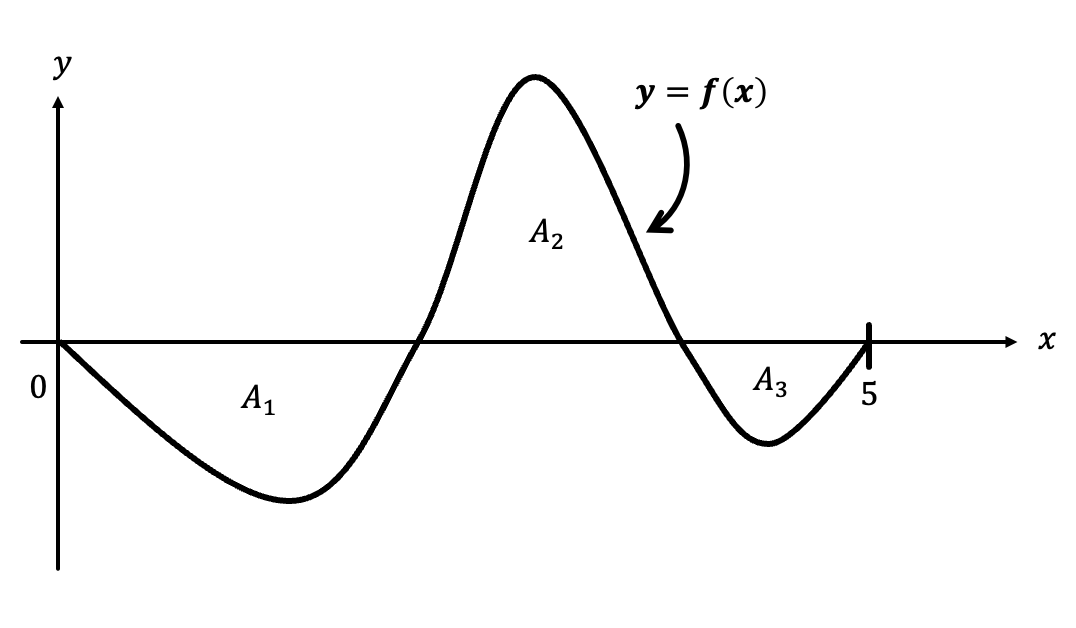
\includegraphics[width=0.7\linewidth]{chapter4/area}

\end{enumerate}
\end{myframe}

\pairofprobsans%
{$\displaystyle \int_{-1}^4 \frac{1}{x^2} \, dx$ }{undefined}
{$\displaystyle \int_{1}^2 x \, dx $ }{$\displaystyle \frac{3}{2}$}

\newpage
\pairofprobsans%
{$\displaystyle \int_0^3 \left( 9-x^2 \right) \, dx$ }{$\displaystyle 18$}
{$\displaystyle \int_0^{\frac{\pi}{3}} \sec^2{(x)} \, dx $ }{$\displaystyle \sqrt{3}$}

\pairofprobsans%
{$\displaystyle \int_1^1 x^2 \, dx$ }{$\displaystyle 0$}
{$\displaystyle \int_4^0 x \, dx $ }{$\displaystyle -8$}

\newpage
\problemans%
{Evaluate the integral $\displaystyle \int_0^6 f(x) dx$ if
	$ \displaystyle f(x) = \begin{cases} 
		x^2 & x < 2 \\
		3x-2 & x\geq 2 
	\end{cases}
	$.
	}%
{$\displaystyle \frac{128}{3}$}

%%%% GUIDES
\qrfigure{chapter4/qr/Definite-Integral}{Scan for guides}
%----------------------


